\documentclass[11pt,a4paper,twoside]{tesis}
% SI NO PENSAS IMPRIMIRLO EN FORMATO LIBRO PODES USAR
%\documentclass[11pt,a4paper]{tesis}

\usepackage{graphicx}
\usepackage[utf8]{inputenc}
\usepackage[spanish]{babel}
\usepackage[left=3cm,right=3cm,bottom=3.5cm,top=3.5cm]{geometry}
\usepackage{sidecap} 
\usepackage{color}
\usepackage{listings}

\graphicspath{ {Images/} }

\setlength{\parindent}{1em}
\setlength{\parskip}{4pt}

\begin{document}

%%%% CARATULA
% Comentar y descomentar según corresponda
%\def\titulo{Licenciada }
\def\titulo{Licenciado }

\def\autor{Fernando Bugni}
\def\tituloTesis{Recolección online de grabaciones para el estudio de las variantes argentinas del español}
\def\runtitulo{Recolección online de grabaciones para el estudio de las variantes argentinas del español}
\def\runtitle{Star Wars: Rebellion and Empire}
\def\director{Agustín Gravano}
\def\codirector{Miguel Martínez Soler}
\def\lugar{Buenos Aires, 2014}
\newcommand{\HRule}{\rule{\linewidth}{0.2mm}}
%
\thispagestyle{empty}

\begin{center}\leavevmode

\vspace{-2cm}

\begin{tabular}{l}

\includegraphics[width=2.6cm]{logofcen.pdf}
\end{tabular}


{\large \sc Universidad de Buenos Aires

Facultad de Ciencias Exactas y Naturales

Departamento de Computaci\'on}

\vspace{6.0cm}

%\vspace{3.0cm}
%{
%\Large \color{red}
%\begin{tabular}{|p{2cm}cp{2cm}|}
%\hline
%& Pre-Final Version: \today &\\
%\hline
%\end{tabular}
%}
%\vspace{2.5cm}

{\huge\bf \tituloTesis}

\vspace{2cm}

{\large Tesis presentada para optar al t\'{\i}tulo de\\
\titulo en Ciencias de la Computaci\'on}

\vspace{2cm}

{\Large \autor}

\end{center}

\vfill

{\large

{Director: \director}

\vspace{.2cm}

{Codirector: \codirector}

\vspace{.2cm}

\lugar
}

\newpage\thispagestyle{empty}


%%%% ABSTRACTS, AGRADECIMIENTOS Y DEDICATORIA
\frontmatter
\pagestyle{empty}
%\begin{center}
%\large \bf \runtitulo
%\end{center}
%\vspace{1cm}
\chapter*{\runtitulo}

\noindent 

El uso de la lengua siempre ha caracterizado a las personas que la utilizan. La forma en como nos comunicamos no sólo posee la información del mensaje a trasmitir, sino que también posee características del hablante. Estas características pueden describir al hablante de distintas formas. Algunas de ellas pueden ser: su cultura, su economía, su región entre otras. 

Particularmente en Argentina no es la excepción. Nuestro país posee una fuerte componente dialéctica en su habla. Esto quiere decir que podemos saber de que lugar proviene el hablante analizando su tonada. Hay varias regiones definidas a través del país. En este trabajo nos enfocaremos en distinguir diferencias entre la región de Córdoba y Buenos Aires. Realizaremos un experimento donde compararemos el habla de cada grupo. Utilizando estos datos analizaremos efectivamente cuales son las características mas predominantes y como repercute esas diferencias en el habla. Por último, mostraremos distintos clasificadores para determinar de que grupo proviene una grabación, analizaremos las atributos mas importantes y testearemos la solución propuesta. 

\bigskip


%\cleardoublepage
%%\begin{center}
%\large \bf \runtitle
%\end{center}
%\vspace{1cm}
\chapter*{\runtitle}

\noindent In a galaxy far, far away, a psychopathic emperor and his most trusted servant -- a former Jedi Knight known as Darth Vader -- are ruling a universe with fear. They have built a horrifying weapon known as the Death Star, a giant battle station capable of annihilating a world in less than a second. When the Death Star's master plans are captured by the fledgling Rebel Alliance, Vader starts a pursuit of the ship carrying them. A young dissident Senator, Leia Organa, is aboard the ship \& puts the plans into a maintenance robot named R2-D2. Although she is captured, the Death Star plans cannot be found, as R2 \& his companion, a tall robot named C-3PO, have escaped to the desert world of Tatooine below. Through a series of mishaps, the robots end up in the hands of a farm boy named Luke Skywalker, who lives with his Uncle Owen \& Aunt Beru. Owen \& Beru are viciously murdered by the Empire's stormtroopers who are trying to recover the plans, and Luke \& the robots meet with former Jedi Knight Obi-Wan Kenobi to try to return the plans to Leia Organa's home, Alderaan. After contracting a pilot named Han Solo \& his Wookiee companion Chewbacca, they escape an Imperial blockade. But when they reach Alderaan's coordinates, they find it destroyed - by the Death Star. They soon find themselves caught in a tractor beam \& pulled into the Death Star. Although they rescue Leia Organa from the Death Star after a series of narrow escapes, Kenobi becomes one with the Force after being killed by his former pupil - Darth Vader. They reach the Alliance's base on Yavin's fourth moon, but the Imperials are in hot pursuit with the Death Star, and plan to annihilate the Rebel base. The Rebels must quickly find a way to eliminate the Death Star before it destroys them as it did Alderaan (aprox. 200 palabras).

\bigskip

\noindent\textbf{Keywords:} War, Rebellion, Wookie, Jedi, The Force, Empire (no menos de 5).

\cleardoublepage
\chapter*{Agradecimientos}

\noindent Lorem ipsum dolor sit amet, consectetur adipiscing elit. Fusce sapien ipsum, aliquet eget convallis at, adipiscing non odio. Donec porttitor tincidunt cursus. In tellus dui, varius sed scelerisque faucibus, sagittis non magna. Vestibulum ante ipsum primis in faucibus orci luctus et ultrices posuere cubilia Curae; Mauris et luctus justo. Class aptent taciti sociosqu ad litora torquent per conubia nostra, per inceptos himenaeos. Mauris sit amet purus massa, sed sodales justo. Mauris id mi sed orci porttitor dictum. Donec vitae mi non leo consectetur tempus vel et sapien. Curabitur enim quam, sollicitudin id iaculis id, congue euismod diam. Sed in eros nec urna lacinia porttitor ut vitae nulla. Ut mattis, erat et laoreet feugiat, lacus urna hendrerit nisi, at tincidunt dui justo at felis. Class aptent taciti sociosqu ad litora torquent per conubia nostra, per inceptos himenaeos. Ut iaculis euismod magna et consequat. Mauris eu augue in ipsum elementum dictum. Sed accumsan, velit vel vehicula dignissim, nibh tellus consequat metus, vel fringilla neque dolor in dolor. Aliquam ac justo ut lectus iaculis pharetra vitae sed turpis. Aliquam pulvinar lorem vel ipsum auctor et hendrerit nisl molestie. Donec id felis nec ante placerat vehicula. Sed lacus risus, aliquet vel facilisis eu, placerat vitae augue. % OPCIONAL: comentar si no se quiere

\cleardoublepage
\hfill \textit{A mi viejo, que me ayuda desde el cielo.}

\hfill \textit{A mi vieja, que gracias a ella soy lo que soy.} 

\hfill \textit{Y a mi hermano, que es el compañero de mi vida.}  % OPCIONAL: comentar si no se quiere

\cleardoublepage
\tableofcontents

\mainmatter
\pagestyle{headings}

%%%% ACA VA EL CONTENIDO DE LA TESIS

\chapter{Introducción}

El uso de la lengua siempre ha caracterizado a las personas que la utilizan. La forma en como nos comunicamos no sólo posee la información del mensaje a trasmitir, sino que también posee características del hablante. Estas características pueden describir al hablante de distintas formas. Algunas de ellas pueden ser: su cultura, su economía, su región entre otras. 

\begin{figure}[h!]
    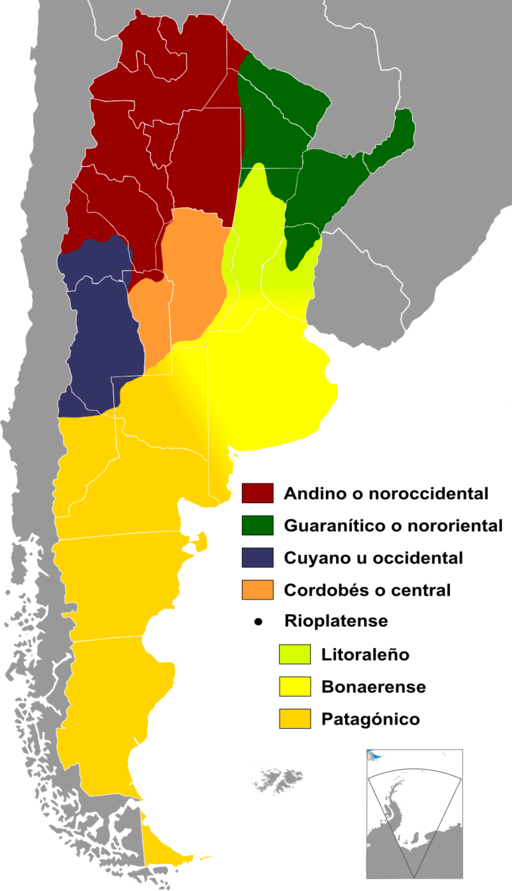
\includegraphics[width=0.5\textwidth]{Dialectos_del_idioma_espanol_en_Argentina} 
    \caption{Dialectos del idioma español en Argentina}
\end{figure}

Particularmente en Argentina no es la excepción. Nuestro país posee una fuerte componente dialéctica en su habla. Esto quiere decir que podemos saber de que lugar proviene el hablante analizando su tonada. Hay varias regiones definidas a través del país. En este trabajo nos enfocaremos en distinguir diferencias entre la región de Córdoba y Buenos Aires. Realizaremos un experimento donde compararemos el habla de cada grupo. Utilizando estos datos analizaremos efectivamente cuales son las características mas predominantes y como repercute esas diferencias en el habla. Por último, mostraremos distintos clasificadores para determinar de que grupo proviene una grabación, analizaremos las atributos mas importantes y testearemos la solución propuesta. 

Vamos a describir las diferencias dialécticas que existen. Las reglas propuestas van a describir como habla la dialéctica de Córdoba. Las reglas son: 

%%\section*{Diferencias entre hablantes}
\subsection*{Regla 1: Localice la sílaba acentuada en la palabra y estirar la silaba anterior}

Cada palabra posee su sílaba acentuada. Para cumplir esta regla se debe estirar la sílaba anterior a esta. Si la sílaba acentuada es la primera de la palabra, entonces no se estira. 

Ejemplo: 'Espectacular' posee su sílaba acentuada en '-lar'. La sílaba anterior, o sea '-cu-' se alarga. 

%%De la regla 1: Se estira en la vocal. 

\subsection*{Regla 2: Aspiración y elisión de /s/}

Para las palabras terminadas en /s/ se debe acortar su duración para Córdoba. 

Ejemplo: 'Pájaros' posee el fonema /s/ al final. Utilizando la dialéctica de Córdoba, la /s/ final sería mas suave que una de Buenos Aires. 

\subsection*{Regla 3: La ‘s’ antes de la ‘c’ o ‘t’ suenan suaves}

La sílaba /s/, que precede a /c/ o /t/, debe sonar suave. 

Ejemplo: 'Mosca' en el dialéctico de Córdoba posee una sílaba más suave en el fonema /s/ que en Buenos Aires. 

\subsection*{Regla 4: La 'c' antes de la 't' no se pronuncia}

La sílaba /c/, que precede a /t/, no se debe pronunciar. 

Ejemplo: 'Doctor' no debe sonar el fonema /c/.

\subsection*{Regla 5: La ‘y’ y ‘ll’ se pasa a ‘i’}

Palabras con el fonema /y/ o /ll/ se pronuncian /i/. 


Ejemplo: 'lluvia' se debe pronunciar utilizando el fonema /i/ 

\subsection*{Regla 6: La ‘r’ no debe sonar. No debe vibrar}

Palabras con el fonema /r/ deben ser suaves y no vibrar. 

Ejemplo: 'Espárrago' debe ser suave en comparación de Buenos Aires. 

Cabe destacar que estas reglas se producen en habla espontánea. No surgen de habla leída. 

Vamos a tomar distintas frases donde aparecen estas reglas y compararlas con la dialéctica de Buenos Aires. 

\chapter{Diseño del experimento}

Analizando el acento de cada ciudad pudimos extraer dichas reglas que describen la diferencia entre cada uno de los dos grupos. Vamos a proponer realizar un experimento para poder extraer la información fonética de estos grupos. El experimento va a poner foco primordialmente en las diferencias antes dichas. La idea sera realizar una serie de actividades donde el hablante sea grabado y esas actividades hagan incapié en las diferencias. Como el acento se potencia cuando se realiza habla espontánea, vamos a querer que el hablante lo diga de forma lo más natural posible. 

Las actividades pensadas a realizar fueron: leer una palabra, leer una frase o describir una image. Dado la dificultad de conseguir hablantes y convocarlos en un mismo lugar físico, vamos a desarrollar una aplicación web capaz de realizar el experimento de forma remota. 

A continuación vamos a describir el experimento en más detalle.

%\section{Motivación}
\section{Actividades}

Nuestro objetivo es extraer la diferencia entre el acento de Córdoba y Buenos Aires. Como dijimos, pensamos tres tipos de grabaciones: leer una palabra, leer una frase, describir una imagen.

Pensándolo más en detalle, nos quedamos con leer una frase. Descartamos leer una palabra porque no lograba darle una entonación interesante. Descartamos describir una imagen ya que las descripciones añaden cierta ambigüedad que hace que las palabras usadas no sean las apropiadas para identificar las diferencias de cada acento.

%Descartamos decir una palabra y decir una imagen por los siguientes motivos. Sobre decir una palabra: uno de los principales objetivos es extraer la espontaneidad del hablante. Realmente si uno dice una palabra no le impregna espontaneidad ya que es una palabra sola y leída. Sobre la imagen: si bien posee mucha espontaneidad puede suceder que la variabilidad sea muy grande. Varios hablantes podrían decir cosas completamente distintas y no podríamos obtener ninguna de las reglas propuestas.

\subsection{Frases conocidas}

Debemos obtener habla espontánea de los hablantes. Es por ello que se nos ocurrió como actividad pronunciar frases popularmente conocidas. Pensamos que al ser muy conocidas el hablante, al haberla pronunciado tanto, vamos a obtener habla expontanea.

%Vamos a querer utilizar frases lo mas conocidas posibles, para que el hablante ya tenga registrada como decirla sin poderle eliminar el acento. De esta forma se quiere obtener habla espontánea.

\section{Diseño teórico}

Para realizar las grabaciones debemos darle a cada hablante una serie de frases a grabar. A esa serie de frases las llamaremos trazas.

\subsection{Descripción de los 2 grupos}
%-Descripción de los 2 grupos. Porque cada uno. Espontaneidad vs Regla 1

Vamos a tener dos formas de grabaciones: frases comunes que tratan de cubrir la espontaneidad (cubriendo las reglas 2 al 5) y frases AMPER que tratan de cubrir el acento barriendo por cada tipo de acentuación (regla 1)

\subsection{Frases utilizadas}

\begin{figure}[h!]
    \centerline{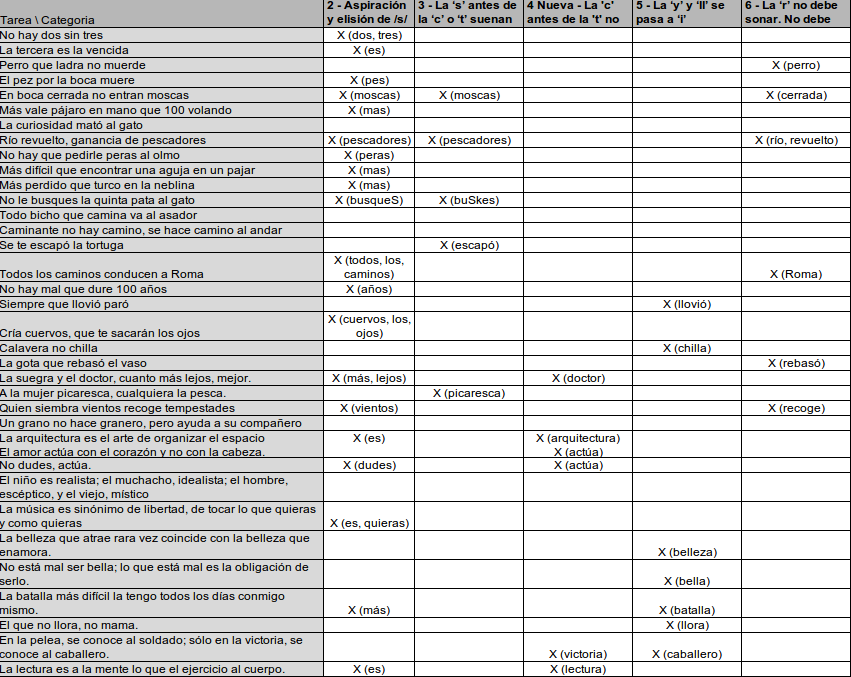
\includegraphics[width=1\textwidth]{frases_inf} }
    \caption{Frases conocidas}
\end{figure}

\begin{figure}[h!]
    \centerline{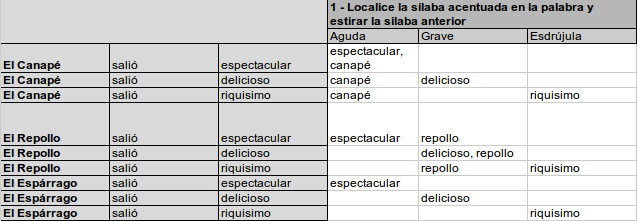
\includegraphics[width=1\textwidth]{reglas_AMPER} }
    \caption{Frases AMPER}
\end{figure}

\subsection{Utilizar AMPER}
Utilizamos este esquema para analizar todas las variantes posibles de la Regla 1. Esta regla es la más conocida y puede aparecer de varias formas. Es por eso que este esquema nos va a resultar muy útil. 

Para el esquema AMPER fijamos un patrón y fuimos cambiando las palabras que utiliza. El esquema AMPER utilizado es: Objeto+” salió “+Adjetivo … donde Objeto puede ser [Canapé. Repollo, Espárrago]. Adjetivo puede ser [espectacular, delicioso, riquisimo]. Utilizamos estas palabras ya que hacen un cubrimiento por la acentuación de cada palabra, o sea pasa por agudas grave y esdrújula. 

%También se agregó “El rábano salió horrible” que posee un acento en la primer sílaba.

\subsection{Intercalando los dos tipos}

Ahora debemos intercalar las trazas de frases comunes con las de Amper. Vamos a agregar 4-5 frases de la traza de frases comunes, luego agregar 1-2 frases del esquema de amper y asi sucesivamente. La idea es no cansar al hablante con frases repetitivas y evitar que sepa de antemano que frase va a tener que grabar.

\subsection{Siempre cada 5 grabaciones:}
La minima cantidad de grabaciones que puede realizar un hablante son 5 grabaciones. Luego se le pregunta si quiere seguir grabando, si dice que si se le agregan otras 5 grabaciones asi sucesivamente hasta llegar a las 40 que es el total de grabaciones.

\section{Generación de trazas}

%Debemos definir qué frases y en que órden se debe decir durante el experimento. Este orden va a tener la condición de que en cada nueva frase agregada vamos a querer cubrir lo mayor posible el porcentaje de cubrimiento de cada una de las reglas. Utilizaremos un algoritmo goloso para generar la traza hasta poder cubrir el 100\% de cada regla.

%La idea del algoritmo para generar trazas se va a basar en utilizar la frase que mayor información aporte en cada paso. No es lo mismo grabar una frase que solo aporta información a la regla 2 que una que aporta a la regla 2, 3, 4. Por ello, en cada paso se va agregando una frase que no fue utilizada y además que aporte la mayor cantidad de información. Es importante aplicar esta idea ya que no sabemos cuanto tiempo va a querer/tener un hablante para realizar el experimento. Utilizando nuestro algoritmo, podemos afirmar que ya con 10 frases grabadas se cubre con todas las reglas propuestas anteriormente. En el gráfico podemos ver el desempeño de nuetro algoritmo. 

Debemos definir qué frases y en que órden se debe decir durante el experimento. Una traza es una lista de las frases que va a grabar un hablante. Sucede que el orden que utilicemos va a ser crucial para tener muestras. No es lo mismo empezar por una frase que sólo referencia a una regla que a varias. Si referencia a varias reglas a la vez, en un sólo audio podremos sacarle más información.

Optamos por tener precalculada las trazas para evitar cálculos innecesarios a la hora de empezar el experimento. Es por eso que guardamos 10000 trazas generadas. Un hablante al empezar se le dará una de estas y grabará sucesivamente en ese orden.

La generación de trazas sigue el siguiente algoritmo:

%todo: Escribir un pseudo codigo de la generación de frases??

Vamos a ponderar las frases que referencien a más reglas. Al generar las trazas vamos a utilizar un contador que nos va a decir cuantas muestras tenemos por cada regla. En cada paso vamos a ver ese contador y vamos a elegir la próxima frase tomandolo en cuenta. Elegiremos la frase que haga referencia a la regla menos grabada en el contador y además que represente a mas de una regla. De esa forma intentamos obtener la mayor cantidad de información posible con pocas grabaciones.

Lo bueno de esto es que para un hablante grabando 10 frases tenemos muestras de todas las reglas. Este es un dato importante ya que maximizamos la cantidad de información de cada frase y le hacemos perder menos tiempo realizando el experimento. Esto se puede ver en el siguiente gráfico.

%todo: grafico de cantidad de frases

\begin{figure}[h!]
    \centerline{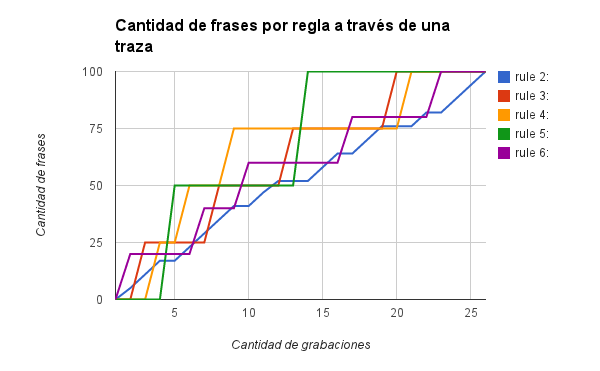
\includegraphics[width=0.9\textwidth]{cant_frases_traza_inf} }
    \caption{Cantidad de frases por traza}
\end{figure}

En conclusión, se grabarán de a 5 frases. Teniendo en cuenta que las últimas 2 corresponderán a el esquema AMPER. 

\chapter{Arquitectura del sistema}

Para poder obtener audios de distintas personas se desarrolló una página web. Esto nos da muchas ventajas ya que nos permite grabar fácilmente desde cualquier lugar.  

La página web esta desarrollada en Django que es un framework para la creación de paginas web. Esta misma necesita una base de datos para guardar cada clase de dominio. En esta base vamos a guardar los datos de cada hablante, las frases a grabar y las trazas principalmente.

\section{Recolección de datos}

Cuando un usuario visita nuestra página, primero le hace llenar un formulario. Este le pregunta: género, fecha de nacimiento y de qué lugar es oriundo. al confirmar los datos, estos son grabados en la base de datos de la aplicación en el servidor. Luego se procede a realizar las grabaciones. 

En la pantalla de grabación el usuario deberá confirmar tener acceso al micrófono que posee en su dispositivo. Una vez hecho esto, puede empezar a grabar. Cada nuevo experimento utiliza una nueva traza. El experimento en total consiste en realizar 40 grabaciones. El hablante va grabando de a 5 frases, cada vez que las termina de grabar ofrece la opción de seguir grabando otras 5 más. De esta forma, aporta el tiempo que puede. Las grabaciones pueden ser escuchadas antes de ser confirmadas por el usuario. Lo importante es que la grabación sea lo mas fehaciente posible.

Cada vez que se confirma una grabación, esta se graba en un archivo wav en el servidor. 

%todo: PONER DATOS TECNICOS DEL TIPO DE WAV

\section{Grabación a través del browser}

Los navegadores actuales no pueden soportar acceder al micrófono directamente. Es por eso que debimos utilizar alguna tecnología alternativa. Buscando encontramos un proyecto llamado WAMI que es una aplicación Flash que nos permite acceder al micrófono a través de JavaScript. Básicamente la aplicación WAMI nos permite grabar un chunk de datos y enviarlo al servidor. El servidor graba ese chunk en un archivo wav.

Pagina de Wami: http://code.google.com/p/wami-recorder/

\section{Requerimientos}

Los requerimientos son básicos: micrófono, conexión a internet. 
Tuvimos problemas sobre el browser que utilizaba. Wami necesita Flash versión 11.04 (chequear) que no se encuentra en los repositorios tradicionales de Ubuntu. De esta manera, los navegadores que utilicen Flash instalado por el sistema operativo Ubuntu no podrán correr. Otros sistemas operativos, como Windows o IOs, no tienen problemas en la versión de Flash instalada. De todas formas el navegador Chrome posee preinstalado dicha versión de Flash, entonces este navegador podía correr perfectamente la aplicación sin importar el sistema operativo.

\section{Administración}

El sistema debe tener datos cargados para estan online recolectando audios. Los minimos datos para poder tener la página funcionando en vivo son los datos de las trazas y la clasificación de los audios. Este cargo de datos se pueden guardar con fixtures del framework Django. Una vez cargado esos datos, los hablantes van a acceder a una url donde van a poder realizar el experimento grabando los distintos audios.

\subsection{Etiquetando audios}

Cuando varias personas terminan el experimento, los administradores pueden acceder a una url donde se puede escuchar cada audio que se va generando. Y si fue exitoso, o sea no esta saturado y no tiene ruidos, puede etiquetarlo con alguna de las etiquetas definidas. Las etiquetadas utilizadas esta vez son: ‘Conservar’,  ‘Sonido saturado’, ‘Mucho ruido de fondo’, ‘Problemas en el habla’. Más adelante veremos como obtener estos audios.

\begin{figure}[h!]
    \centerline{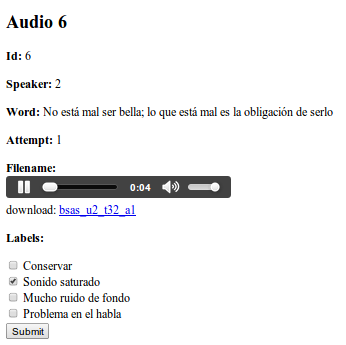
\includegraphics[width=0.5\textwidth]{categorizando_audios} }
    \caption{Categorizando audios}
\end{figure}

\subsection{Backups automáticos}

El sistema posee backups automáticos generados a la noche automáticamente. Los backups consisten en un dump de la base de datos y de sincronizacion de los audios con una carpeta de backup. De esta forma, se guardan todos los datos cada día, y los audios quedan a salvo.

\subsection{Export de wavs y csv}

Luego de obtener varios audios podemos exportar todos los datos a traves de urls. Utilizamos distintas urls que nos van a permitir bajarnos los audios etiquetados. Por ejemplo si accedemos a /conservados vamos a bajar los audios etiquetados de esa forma. Idem para las demas. Tambien se pueden bajar todos los audios sin etiquetas. Sobre la base de datos, se pueden bajar todo el modelo de datos a formato csv.

\section{Filtrado de audios}

Debemos evitar grabar audios saturados. Para ello se nos ocurrió sensar el volumen de la grabación cuando sucede la misma. El resultado es una serie de valores entre 0 a 100. Sobre estos valores vamos a calcular el máximo y el mínimo. Si el primero es mayor a un cierto umbral (o sea mayor a 80) quiere decir que en la grabación se saturó en algún momento. Si el mínimo es menor a un cierto umbral (o sea menor a 20 por ejemplo) quiere decir que hay mucho sonido ambiente. En cualquiera de los dos casos podemos pedirle al usuario que grabe devuelta el experimento. De esta forma podemos filtar audios que no nos servirán para reconocer el acento.

Si bien esta característica esta fue programada, no fue utilizada en la recolección de datos. El motivo fue que queriamos chequear cuan bien funcionaba la herramienta sin filtros y con completa participación de los usuarios. Otro motivo fue la paciencia de los hablantes. Puede suceder que al tratar de grabar no logre un ambiente beneficioso para grabar. Esto quiere decir que aunque quiera grabar el filtro rechace todos sus audios. Esto no lo queremos como primer experimento del framework. Por eso optamos por aceptar todos sus audios.

Para los audios que salieron saturados, más adelante vamos a realizar un estudio para intentar sacarles el ruido y de esta forma intentar rescatarlos.

\section{Varias grabaciones por frase}

Siguiendo con la idea de tener la mejor grabación de cada hablante, le dimos la opción a cada hablante de que después de grabar un audio de una frase puedan escucharse como quedó. Esto requiere un ida y vuelta entre el cliente (navegador) y el servidor. Al grabar, el cliente manda un mensaje HTTP POST para el servidor con los datos de grabación. Las frases son cortas entonces no es necesario preocuparse por la longitud del paquete. Cuando el cliente quiere escucharlo envía un mensaje GET a ese mismo audio anteriormente grabado. El servidor envía la grabación y es reproducida en el cliente. Esta ida y vuelta de la grabación podría ser optimizada para que la grabación pueda ser escuchada sin tener interacción con el servidor. En nuestro experimento, no tuvimos problemas graves en lo que respecta a latencias pero si es un punto débil del sistema.

A cada hablante le dimos la opción que pueda escuchar y volver a grabar la frase cuantas veces quisiera. Esto lo hicimos para poder detectar cual es el disparador que hace que diga mal una frase. Puede resultar interesante analizar los anteriores audios y porque se queda con el último.

\chapter{Extracción de datos}

\section{Alineación forzada}

Gracias a nuestra página web se van a poder obtener distintas muestras de Córdoba y Buenos Aires. Pero ¿Cómo podemos analizar estos audios correctamente?. Un archivo wav, como los que captura la página cada una de las pruebas, posee muchísima información. Es por esto que debemos seleccionar correctamente que partes de la información nos sirve y que partes podemos descartar. Y además, un dato muy relevante, es que esta selección no debe tener que ser realizada con intervención de un humano. Ya que, si tenemos muchos audios tendríamos que hacerlo uno por uno y sería un trabajo muy arduo.

Las partes que debemos extraer de los audios son las partes donde se encuentran la diferencias de cada regla descripta anteriormente. Debemos tener una herramienta que nos permita obtener esas pequeños pedazos de audios para analizar sus diferencias. Luego de buscar bastantes, nos topamos con una librería llamada ProsodyLab Aligner (http://prosodylab.org/tools/aligner/). Su función es realizar alineaciones automáticas utilizando Hidden Markov Model. Una de las ventajas que posee es que puede utilizarse para cualquier idioma. Sólo se necesita una hora de audio grabado y un diccionario fonético sobre las palabras a reconocer. 

La hora de grabación la debíamos cumplir recolectando grabaciones de la página web. Esta meta era posible de realizar. La creación de un diccionario era más complicado, ya que debía ser en español. Gracias a Laboratorio de Investigaciones Sensoriales - INIGEM que nos prestó su diccionario pudimos utilizar esta herramienta. El diccionario fonético nos provee para cada palabra los distintos fonemas que la componen. De esta manera, se puede realizar una alineación acorde al español.

\subsection{Diccionario TranscriptorFonetico2 del LIS}

Un diccionario fonético es básicamente un listado con las palabras que utilizamos y su división en fonemas. Es importante esto ya que va a ser usado por el alineador para describir los fonemas de cada palabra.

\section{Extracción de atributos}

En esta sección vamos a analizar como extraer cada uno de los atributos que planteamos en cada regla.

\subsection{Implementación}

La extracción de datos fue realizado en el lenguaje Python. Elegimos ese ya que es un lenguaje de fácil de programar y tiene muchas librerías útiles para este tipo de casos. Utilizamos una muy conocida llamada Numpy. Esta es una librería para el calculo preciso en aplicaciones científicas.

El extractor posee como input los archivos .wav y los archivos textgrid que corresponden a las alineaciones temporales de cada fonema en cada audio. El extractor se debe ejecutar después de la alineación. 

\begin{figure}[h!]
    \centerline{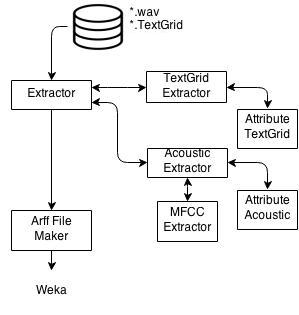
\includegraphics[width=0.5\textwidth]{diagrama_workflow} }
    \caption{Diagrama workflow}
\end{figure}


El ProsodyLab-Algner al finalizar una alineación nos devuelve un archivo donde se encuentra como fueron realizadas esas alineaciones. Este archivo se llama '.SCORES' y en el son lista todos los audios seguidos de un valor. Este valor nos permite ver la verosimilitud de las alineaciones. Si una alineación fue similar a otra va a tener aproximadamente un valor similar. En cambio, si posee una alineación muy distinta va a tener valores muy distintos. Este va a ser el primer filtro para el extractor. Ordenando los audios en esta escala notamos que los menores poseen alineaciones malas, entonces definimos un umbral para el cual aceptar y rechazar la alineación.

Luego de esto, el extractor va a correr un conjunto de funciones que van a extraer cada uno de los atributos. Este conjunto de funciones se dividen en dos: las que computan atributos temporales y las que computan atributos acústicos. Veamos cada uno:

\subsection{Atributos temporales}

Corresponden a los atributos de duración en los fonemas y la sílabas de cada frase. Para calcularlos utilizamos como input el textgrid generado en la alineación. Básicamente estas funciones recorren el textgrid buscando un patrón en particular y lo miden.

Las mediciones son normalizadas de dos formas: primero una normalización normal utilizando:

\hspace{2cm} \[\frac{X - \mu }{ \sigma }\]

y luego otra pensando que $\mu = 0$. 

\hspace{2cm} \[\frac{X}{ \sigma }\]

Esta ultima tiene el nombre de half normal distribution.

%todo: agregar imagen explicando normalización

Vamos a dividir el grupo de los atributos temporales en dos grupos: fonéticos y silábicos. Cada grupo calcula igual la normalización pero uno va a tener en cuenta fonemas y otro sílabas. Veamos cuales son:

\subsubsection{Atributos fonéticos}

\begin{itemize}
    \item \textbf{Duración de la 'kt':} con este atributo vamos a buscar el patrón 'kt' en las frases y luego a medir normalizando de las dos formas el fonema 'k'.  
    \item \textbf{Duración de la 'sc':} ídem con 'sc' y midiendo el fonema 's'.
    \item \textbf{Duración de la 'll':} buscamos el patrón 'll' y lo medimos normalizandolo.
    \item \textbf{Duración de la 'rr':} ídem para 'rr'.
    \item \textbf{Duración de la 's' final:} Ídem para las 's' de final de palabra.
    
    \item \textbf{Duración de cada fonema:} este atributo mide la cantidad de fonemas y realiza un promedio. Este no se realiza normalización.  
    \item \textbf{Duración de cada vocal:} contabilizamos cada vocal y luego realizamos su normalización utilizando la duración de cada fonema.
    \item \textbf{Duración de cada consonante:} Ídem para consonantes. 
\end{itemize}

\subsubsection{Atributos silábicos}

Vamos a hacer un análisis de la sílabas. Los atributos que usamos son:

\begin{itemize}
    \item \textbf{Duración de la sílaba acentuada:} en cada una de las frases vamos a buscar la sílaba acentuada de cada palabra, mediremos su duración y normalizaremos con las demás sílabas.
    \item \textbf{Duración de la sílaba anterior a la acentuada:} realizamos el mismo calculo anterior pero con la sílaba previa a la acentuada. 
\end{itemize}

Estos atributos usamos para poder medir fuertemente la Regla 1, que esta es la más resaltada de la tonada cordobesa. 

\subsection{Atributos acústicos}

Los atributos acústicos utilizan las propiedades de los wavs grabados. Para ello debimos extraer información con algún método que permita medirlos. Elegimos el calculo de MFCC ya que tiene relación directa con la percepción auditiva humana. 

\subsubsection{Mel Frequency Cepstral Coefficients}

%http://practicalcryptography.com/miscellaneous/machine-learning/guide-mel-frequency-cepstral-coefficients-mfccs/

La forma en que hablamos se produce por varias articulaciones. Algunas de ellas pueden ser: dientes, lengua, traquea etc. Estas articulaciones trabajan de forma tal para producir el sonido. Pero también funcionan para darle forma y aplicarle un filtro al sonido producido. Si sabemos correctamente que filtro se le aplica, podremos saber que sonido produce. La forma y el filtro asociado nos muestra donde esta la fuerza en el fonema.

Las señales de audio cambian constantemente poseen muchas variaciones. En periodos cortos de tiempo estas variaciones se reducen. Vamos a dividir todo el audio en pequeños frames para calcular en ellos los coeficientes. El tamaño de cada frame esta entre 20-40 ms. Si la variación es menor a este frame, habrá pocas pruebas para tenerla en cuenta y entonces la descartaremos.

Luego para cada frame se calcula el espectro de frecuencia. Esto se viene motivado por un órgano que se encuentra en la oreja llamado Cóclea. Este vibra de diferente forma al llegarle cada frecuencia del sonido. Al vibrar, activa nervios que representan las distintas frecuencias que escuchamos. Dividir el sonido en períodos intenta mostrar que frecuencias están activas.

El Cóclea no reconoce diferencias entre dos frecuencias muy cercanas. Esto se incrementa mientras más alejada esta esa frecuencia. Para representar esta idea se utiliza un filtrado por escala de Mel. 

%http://i.stack.imgur.com/YUH48.gif

Mientras mas aumentamos la frecuencia, mas anchos son los filtros aplicados. Lo importante es ver cuanta energía hay en las frecuencias involucradas en el filtro. Luego que tenemos la energía de estos tramos le aplicamos el logaritmo. Esto se ajunta mejor a como escucha el oído. Para finalizar se computa DCT de las energías filtradas. 

Debemos extraer datos de los wavs grabados. Para ello debemos analizarlos y que ese análisis nos de una medida que pueda compararse. El análisis debe tener en cuenta como lo percibe un humano. Las frecuencias de Mel ayudan a describir la percepción humana del lado de las frecuencias que escucha. 

\subsubsection{Implementación}

Para realizar el calculo de estos coeficientes se utilizó un script en Matlab. El extractor necesita estos valores para cada audio a extraer. Es por eso que se conecta con Matlab a través de un wrapper para calcular el script y luego continuar con la extracción.

\chapter{Datos obtenidos}

En este capitulo vamos a analizar los datos obtenidos.

\section{Audios recolectados via web}

Los audios recolectados tuvieron algunos problemas al grabarse. El principal problema fue que el ambiente que utilizó cada hablante no estaba en silencio como para hacer una buena grabación. Muchos errores surgieron en esa dirección. Otros errores comunes pero no tan frecuentes fueron: interpretaciones erróneas de la consigna, errores de volumen del micrófono, saturación etc.. 

\subsection{Mediciones}

Los audios fueron escuchados para determinar si se realizó correctamente. Los fuimos clasificando en: Conservar, Sonido saturado, Mucho ruido de fondo, Problema en el habla. Esta clasificación fue empírica, o sea no realizando ningún análisis sino que escuchando manualmente cada una. La cantidad de cada clase fue la siguiente

\begin{table}[h]
\centering
\begin{tabular}{|l|c|c|c|c|}
\hline
\textbf{}  & \textbf{Bs.As. } & \textbf{Cba.} & \textbf{Total} \\ \hline
\textbf{Conservar}  & 222 & 105 & 327 \\ \hline
\textbf{Problemas en el habla}  & 33 & 15 & 48 \\ \hline
\textbf{Mucho ruido de fondo}  & 2 & 12 & 14 \\ \hline
\textbf{Sonido saturado}  & 2 & 0 & 2 \\ \hline
\end{tabular}
\end{table}

Algo importante de ver es que los datos obtenidos están desbalanceados. No pudimos obtener la misma cantidad de audios para los dos grupos. Esto se va a reflejar en la clasificación y en el análisis posterior.

\subsection{Errores comunes}

Las categorías establecidas anteriormente describen los errores comunes mas frecuentes. Podemos observar que del total de 391 grabaciones, 64 tuvo algún problema. Este es alrededor del 16\% de los audios grabados. Es un número alto para ser un experimento guiado. 

La gran causa de este número es la faltante de un chequeo en el mismo momento que va grabando cada uno de los audios. La idea sería analizar el audio grabado y rechazarlo si no supera un nivel aceptable auditivo. Esto puede implementarse de varias formas. Una posible sería cuando esta grabando sensar el volumen del micrófono cada una cierta cantidad de tiempo, por ejemplo 1 segundo. Si en ese sensado el volumen no se encuentra entre rango máximo y mínimo de volumen, descartar el audio y pedirle al hablante que vuelva a grabar. 

%todo: esto nose si va mejor en Trabajos Futuros
También se le podría dar mas información al hablante. Sabiendo que el micrófono tuvo un pico de volumen se podría pedirle al hablante que no hable tan fuerte. Ídem si habla muy bajo. Otras posibles soluciones a este problema es analizar antes de empezar el experimento si el sonido ambiente es muy alto o no. Y luego de ello aceptar una grabación nueva. Todas esas soluciones e pueden realizar en la aplicación web sin intervenir en el server.

Para análisis mas precisos se puede aplicar mejores filtros cuando llega la grabación del lado del servidor. Cuando llega el mensaje del audio al servidor, este ya puede obtener el wav y realizarle todo tipo de análisis mas precisos. Recordemos que el servidor esta implementado en Python que posee muchas librerías útiles para el análisis de audios. Al momento de terminar el análisis del audio en cuestión, deberá enviar la respuesta al hablante informándole si se debe realizar devuelta la grabación o si fue exitosa. Es importante notar que esta solución necesita buena conexión para el server. 

Vamos a continuar con el análisis basándonos en los audios clasificados como Conservados. Luego trataremos de realizar algún análisis para reutilizar algunos de estos que tuvieron algún problema. 

\section{Alineación forzada}

El alineador automático no realiza su función de forma perfecta. Sucede que muchas veces alinea mal. 

\begin{figure}[h!]
    \centerline{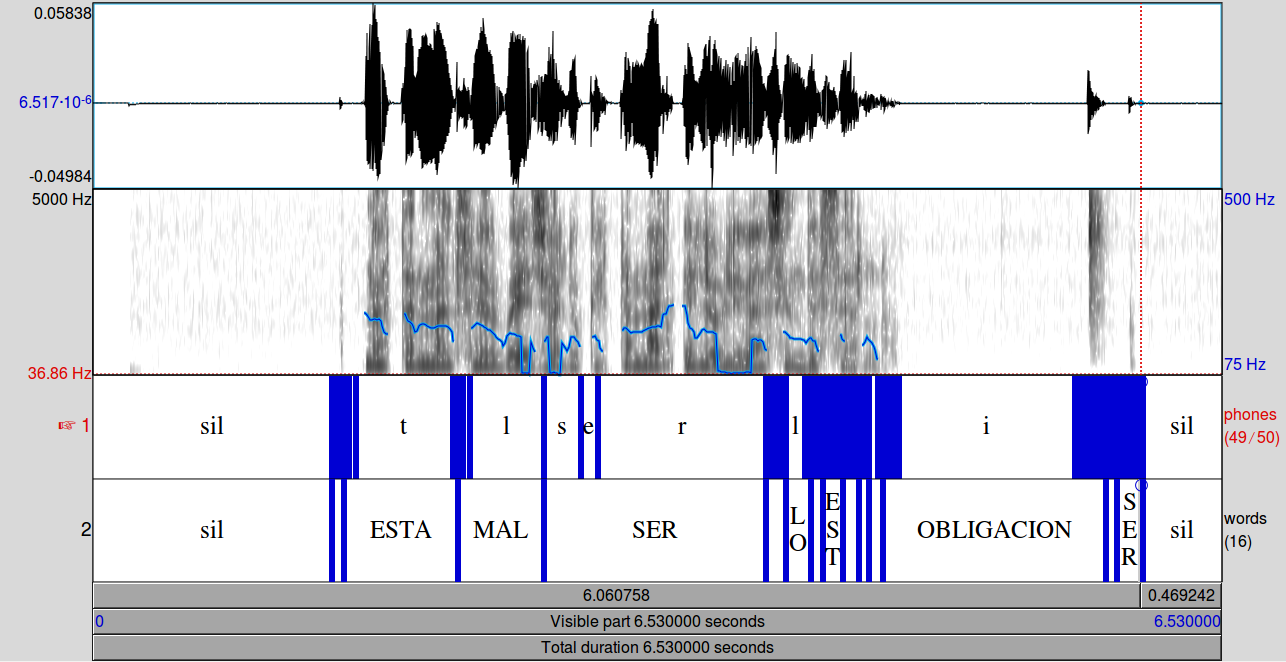
\includegraphics[width=0.8\textwidth]{alineacion_mala_inf} }
    \caption{Alineación mala}
\end{figure}


\subsection{Errores comunes}

Es muy importante descartar los audios mal alineados ya que sino cuando los procese el extractor nos darían información errónea. Fuimos chequeando cada audio y analizando si la alineación fue correcta. Los errores mas comunes fueron:

\begin{itemize}
    \item \textbf{Ruido de fondo:} los casos donde el alineador se comporta de peor manera son los que se escuchan ruido de fondo. En esos casos las alineaciones resultan muy malas. Lamentablemente en nuestro caso esto es muy común. 

    \item \textbf{Mouse click al finalizar:} sucede que el ambiente donde los hablantes realizaban las grabaciones no estaba bien aislado. Pasó en muchas oportunidades que el click de finalizar del mouse se grabó como parte final de la grabación. Ese sonido se grabó y afectó la alineación de forma tal que se tomaba como habla.
    
\begin{figure}[h!]
    \centerline{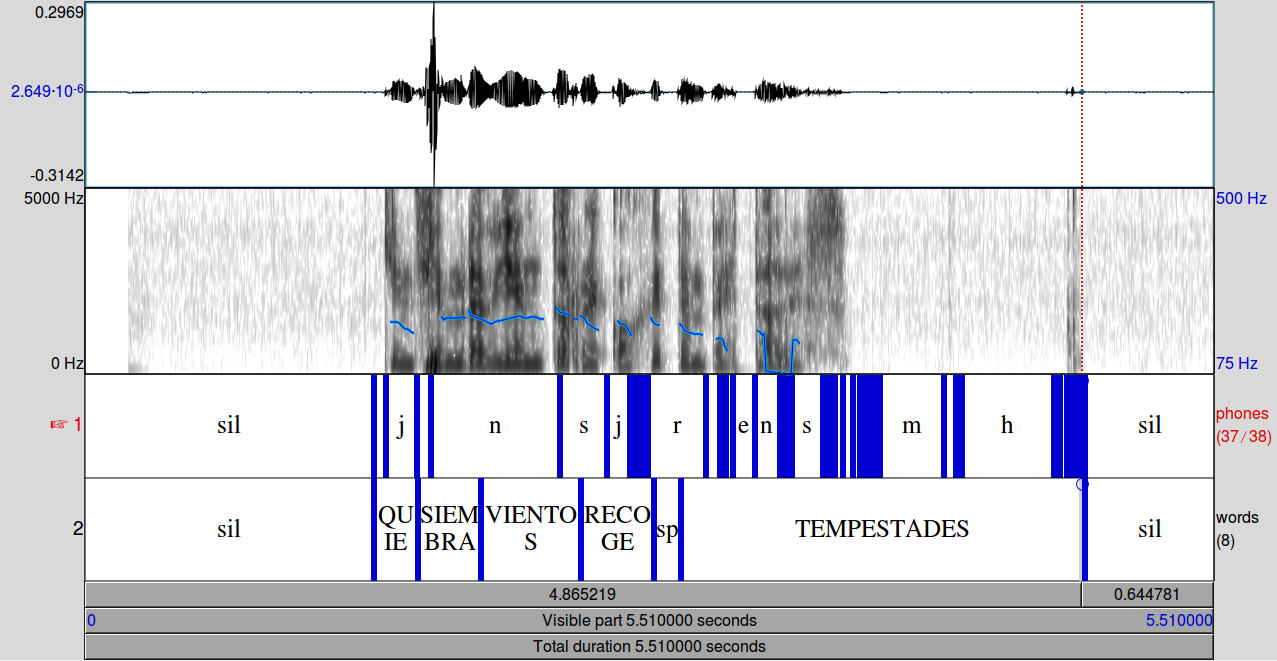
\includegraphics[width=0.8\textwidth]{click_al_final_inf} }
    \caption{Click al final}
\end{figure}


    \item \textbf{Saturación del micrófono:} el volumen del micrófono es configurado por el hablante. Es por ello que debemos confiar en su buena voluntad. Sucede que muchas veces la grabación fue buena pero al final tuvo una entonación mas mucho mas fuerte que las demás, haciendo que posteriormente la alineación no sea precisa.

    \item \textbf{Estiramiento de la /s/ final:} en varias oportunidades se quiso exagerar la entonación. Las frases finalizadas en /s/ fueron grabadas en muchos casos sosteniendo ese fonema por tiempo prolongado. A pesar de que fue alineado correctamente en toda su duración, este fue llevado a una duración entendible. El problema que surgió en estos casos fue que el hablante no supo pronunciar la frase de la forma mas natural posible. Este fue el motivo por el cual se modificó.
\end{itemize}

\section{Corrección de errores}

Para corregir los errores descriptos debimos chequear cada uno de los textgrids. Los resultados de la cantidad de textgrid corregidos son:

\begin{table}[h]
\centering
\begin{tabular}{|l|c|c|c|c|}
\hline
\textbf{}  & \textbf{Bs.As. } & \textbf{Cba.} & \textbf{Total} \\ \hline
\textbf{Modificados}  & 101 & 88 & 189 \\ \hline
\textbf{Correctos sin modificación}  & 119 & 2 & 121 \\ \hline
\end{tabular}
\end{table}

%todo: leer bien el mail de prosodylab
Esta forma se realizó ya que eran pocos audios. Otro modo de hacer esto pero de forma automática puede ser de la siguiente forma. Cuando se realiza la alineación, se crea un archivo llamado .SCORES. Este archivo posee los valores de verosimilitud de cada alineación. Entonces este archivo podría servir para definir si un audio esta bien alineado. Si la alineación superó un  umbral pre-configurado, el audio estará bien alineado y se podrá utilizar para el estudio, sino el audio se descartará. Vale aclarar que esto puede tener falsos positivos.

\subsection{Disminución del ruído con Sox}

\chapter{Análisis}

Vamos a mostrar los resultados que obtuvimos luego de realizar la extracción.

\section{Baseline}

No hay ningún trabajo que trate de distinguir entre porteños y cordobéces a partir de su habla. Es por eso que el baseline se va a determinar a través de algoritmo dummy.

Imaginemos que tenemos un algoritmo que siempre elige un mismo grupo, por ejemplo Buenos Aires. Este algoritmo utilizando nuestros datos tendría una performance buena. Al tener más hablantes de Buenos Aires que de Córdoba en nuestro set de datos acertaría más del 50\% de las veces. 

En promedio va a tender a (Completame XX)\% de efectividad. Esto utilizando la Ley de los Grande Números nos determinaría que la esperanza de elegir a un hablante de Buenos Aires va a ser de  (Completame XX)\%. Este es el porcentaje a superar. 

%Pensemos que para determinar si una persona corresponde a alguno de los grupos vamos a tirar una moneda. Empíricamente podemos afirmar que en promedio la probabilidad de que salga algún grupo es 1/2. Gracias a la Ley de los Grandes Números podemos afirmar que, para valores grandes, esto va a tender a la Esperanza. Entonces, si nosotros queremos identificar un hablante utilizando el azar nos dará el 50\% de efetividad.

%Cabe aclarar que nuestro set de datos no esta debidamente balanceado. Tuvimos más grabaciones de Buenos Aires que de Córdoba. Es por eso que el entrenamiento también va a ser desbalanceado. Por este motivo puede suceder que al clasificar a un hablante en un test se obtenga mejores resultados para características de Buenos Aires que de Córdoba. Lamentablemente eso es una problemática de los datos obtenidos.

Cabe aclarar que si nuestro set de datos estuviera debidamente balanceado este porcentaje no sería tan alto. Lo ideal sería poder tener muestras balanceadas. Al tener este desbalance, puede suceder que al clasificar a un hablante en un test se obtenga mejores resultados para características de Buenos Aires que de Córdoba. Lamentablemente eso es una problemática de los datos obtenidos.

Utilizamos la herramienta de machine learning Weka para poder hacer el análisis. Esta nos provee un clasificador dummy descripto anteriormente. Este se llama ZeroR que es el algoritmo que siempre elige el mayor grupo.

\section{Modelo de testing}

La complejidad del problema y la forma en que fue realizado el experimento nos lleva a tener que descartar un modelo de testing común. Si utilizamos un modelo estándar deberíamos dividir los audios en 2 grupos, uno lo usaríamos para entrenar y otro para testear. Podría surgir el problema de que un hablante tenga audios en el conjunto de training y en el de testing. En ese caso el test sería erróneo ya que estaríamos entrenando con datos que luego serían testeados.

Para evitar este inconveniente debímos tomar en cuenta los hablantes a la hora de dividir los grupos. Vamos a dividir los grupos de train y test eligiendo al azar hablantes. Cuando tomemos un hablante al azar, debemos agregar todos sus audios grabados. En el siguiente pseudocódigo se explica la metodología. 

\lstset{ %
language=C++,                % choose the language of the code
basicstyle=\footnotesize,       % the size of the fonts that are used for the code
numbers=left,                   % where to put the line-numbers
numberstyle=\footnotesize,      % the size of the fonts that are used for the line-numbers
stepnumber=1,                   % the step between two line-numbers. If it is 1 each line will be numbered
numbersep=5pt,                  % how far the line-numbers are from the code
backgroundcolor=\color{white},  % choose the background color. You must add \usepackage{color}
showspaces=false,               % show spaces adding particular underscores
showstringspaces=false,         % underline spaces within strings
showtabs=false,                 % show tabs within strings adding particular underscores
frame=single,           % adds a frame around the code
tabsize=2,          % sets default tabsize to 2 spaces
captionpos=b,           % sets the caption-position to bottom
breaklines=true,        % sets automatic line breaking
breakatwhitespace=false,    % sets if automatic breaks should only happen at whitespace
escapeinside={\%*}{*)}          % if you want to add a comment within your code
}
\begin{lstlisting}
    Generador de Test:
    Input: conjunto audios
    Output: < conjunto train, conjunto test >
    train <- audios
    test <- {}
    mientras percentage < 0.1:
        hablante_BsAs <- Elegir al azar(audios)
        grabaciones_BsAs <- ObtenerGrabaciones(hablante_BsAs, audios)
    
        hablante_Cba <- Elegir al azar(audios)
        grabaciones_Cba <- ObtenerGrabaciones(hablante_Cba, audios)
    
        tests <- tests U grabaciones_BsAs U grabaciones_Cba
        train <- train - grabaciones_BsAs - grabaciones_Cba
    
        percentage <- Tam(test) / Tam(train) 
    
    Devolver <train, test>
\end{lstlisting}

Este proceso lo debemos realizar 10 veces para poder evitar que hayamos tenido suerte al generar el test. Luego de generado estos 10 pares de grupos de train y test vamos a utilizarlos para entrenar clasificadores.

\section{Clasificadores}

Vamos a entrenar varios clasificadores para poder determinar si el análisis de atributos que realizamos aporta mayor información a la hora de detectar un hablante. Los clasificadores propuestos son: JRip, J48, Function SMO, Naive Bayes. Más adelante decribiremos los parametros utilizados para cada uno.

\section{Tests estadísticos}

Vamos a utilizar los resultados de cada clasificador para ver si los resultados son significativamente relevantes. Los resultados que vamos a utilizar van a ser el vector resultante de los 10 grupos de tests utilizando el clasificador ZeroR contrastado con algún clasificador más sofisticado, por ejemplo: JRip, J48, Function SMO, NaiveBayes.
Para ello vamos a realizar dos principales tests: Wilcoxon signed-rank y Test de Student. 

\subsection{Wilcox Test}

Primero realizaremos Wilcox Test ya que necesita menos presunciones. Para realizar este test debemos cumplir que:

\begin{itemize}
    %Data are paired and come from the same population.
    \item Los datos son presentados de a pares y vienen de la misma población: esto sucede gracias a como armamos los tests. La población también siempre es la misma.
    %Each pair is chosen randomly and independently.
    \item Cada par es elegído de forrma azarosa y independiente del resto: cada grupo generado para testing esta armado de forma azarosa ya que la elección de cada hablante se realiza de esta forma.
    %The data are measured at least on an ordinal scale, but need not be normal.
    \item Los datos estan medidos sobre una escala ordinal y no necesariamente debe provenir de una distribución Normal: esta caracteristica es fundamental ya que no estamos seguros que nuestros datos provengan de una distribución Normal.
\end{itemize}

El input del mismo va a ser el vector resultante del test baseline ZeroR con el vector de los demás clasificadores. Las hipótesis van a ser:

\vspace{0.5cm}
\hspace{2cm}Ho: Clasificador alternativo no es mejor que ZeroR
\vspace{0.25cm}

\hspace{2cm}H1: Clasificador alternativo es mejor que ZeroR
\vspace{0.5cm}

donde Clasificador alternativo se refiere a los demás clasificadores. 
Cada uno de los tests nos va a dar un p-valor.
Si este es mayor 0,05 No hay evidencia suficiente para determinar que el clasificador alternativo es mejor.
Si de lo contrario, es menor Si podemos rechazar Ho y asegurar que el alternativo es mejor. 

Luego chequearemos si nuestra muestra es de distribución Normal. Si es ese el caso haremos el Test de Student. Para chequear Normalidad vamos a utilizar el test de Shapiro-Wilk.

\subsection{Análisis Shapiro-Wilk Test}

%todo: pensar si debo explicar todo el metodo o no hace falta
%http://es.wikipedia.org/wiki/Test_de_Shapiro%E2%80%93Wilk

%En estadística, el Test de Shapiro–Wilk se usa para contrastar la normalidad de un conjunto de datos. Se plantea como hipótesis nula que una muestra x1, ..., xn proviene de una población normalmente distribuida. Fue publicado en 1965 por Samuel Shapiro y Martin Wilk.1 Se considera uno de los test más potentes para el contraste de normalidad, sobre todo para muestras pequeñas (n<30).

El Test de Shapiro-Wilk lo utilizamos para notar la normalidad del conjunto de datos. Lo utilizamos ya que posee un buen desempeño en pequeñas muestras.

%Interpretación: Siendo la hipótesis nula que la población está distribuida normalmente, si el p-valor es menor a alfa (nivel de confianza) entonces la hipótesis nula es rechazada (se concluye que los datos no vienen de una distribución normal). Si el p-valor es mayor a alfa, no se rechaza la hipótesis y se concluye que los datos siguen una distribución normal.

Planteamos como hipótesis nula que la población esta distribuida de forma normal, aplicamos el estadístico de este test y si el p-valor nos da mayor a 0,05 entonces la hipótesis nula es rechazada. Si en cambio es menor a 0,05 no se puede rechazar Ho.

Este test se realiza individualmente para cada vector resultado. O sea, debemos chequear que los resultados de ZeroR para ver si su distribución se asemeja a la distribución Normal. Esto para cada resultado de los clasificadores. Si ambos tuvieron p-valor > 0,05, por ejemplo ZeroR y J48, se puede realizar el Student Test. 

\subsection{Student Test}

%En estadística, una prueba t de Student, prueba t-Student, o Test-T es cualquier prueba en la que el estadístico utilizado tiene una distribución t de Student si la hipótesis nula es cierta. Se aplica cuando la población estudiada sigue una distribución normal pero el tamaño muestral es demasiado pequeño como para que el estadístico en el que está basada la inferencia esté normalmente distribuido, utilizándose una estimación de la desviación típica en lugar del valor real. Es utilizado en análisis discriminante.

%A t-test is any statistical hypothesis test in which the test statistic follows a Student's t distribution if the null hypothesis is supported. It can be used to determine if two sets of data are significantly different from each other, and is most commonly applied when the test statistic would follow a normal distribution if the value of a scaling term in the test statistic were known. When the scaling term is unknown and is replaced by an estimate based on the data, the test statistic (under certain conditions) follows a Student's t distribution.

Para los vectores que poseen una distribución Normal vamos a aplicarle este test. Este nos provee una forma de determinar si dos conjuntos de test son significativa mente distintos. De la misma forma que planteamos la hipótesis de Wilcox test, este va a tener las mismas hipótesis. O sea: 

\vspace{0.5cm}
\hspace{2cm}Ho: Clasificador alternativo no es mejor que ZeroR
\vspace{0.25cm}

\hspace{2cm}H1: Clasificador alternativo es mejor que ZeroR
\vspace{0.5cm}

La ventaja de usarlo es que, al saber que distribución representa, vamos a ser mas precisos a la hora de calcular su p-valor. Aplicando el estadístico vamos a obtener un p-valor. De la misma forma, si este es mayor a 0,05 no hay evidencia suficiente para rechazar Ho. De lo contrario, si hay evidencia y rechazamos Ho.

\section{Resultados}

Todos tests fueron realizados utilizando R versión 3.0.1.

\subsection{Clasificadores}
%tabla de weka comparando cada uno de los clasificadores: ZeroR, JRIp, J48, FSMO, NaiveBayes
Los resultados para los distintos clasificadores fueron:

\begin{table}[h]
\centering
\begin{tabular}{|l|c|c|c|c|c|c|}
\hline
\textbf{}  & \textbf{ZeroR} & \textbf{JRip} & \textbf{J48} & \textbf{Function SMO} & \textbf{NaiveBayes} \\ \hline
\textbf{Test 1}  & 0 & 0 & 0 & 0 & 0\\ \hline
\textbf{Test 2}  & 0 & 0 & 0 & 0 & 0\\ \hline
\textbf{Test 3}  & 0 & 0 & 0 & 0 & 0\\ \hline
\textbf{Test 4}  & 0 & 0 & 0 & 0 & 0\\ \hline
\textbf{Test 5}  & 0 & 0 & 0 & 0 & 0\\ \hline
\textbf{Test 6}  & 0 & 0 & 0 & 0 & 0\\ \hline
\textbf{Test 7}  & 0 & 0 & 0 & 0 & 0\\ \hline
\textbf{Test 8}  & 0 & 0 & 0 & 0 & 0\\ \hline
\textbf{Test 9}  & 0 & 0 & 0 & 0 & 0\\ \hline
\textbf{Test 10} & 0 & 0 & 0 & 0 & 0\\ \hline
\end{tabular}
\end{table}

donde Test 1 corresponde al primer par < conjunto train, conjunto test > y así sucesivamente.

\subsection{Wilcox y Student Test}

Vamos a mostrar los resultados de estos tests estadísticos.

\begin{table}[h]
\centering
\begin{tabular}{|l|c|c|c|c|c|c|}
\hline
\textbf{}  & \textbf{Student Test} & \textbf{Wilcox Test} \\ \hline
\textbf{ZeroR y JRip}  & 0 & 0 \\ \hline
\textbf{ZeroR y J48}  & 0 & 0 \\ \hline
\textbf{ZeroR y NaiveBayes}  & 0 & 0 \\ \hline
\textbf{ZeroR y Function SMO}  & 0 & 0 \\ \hline
\end{tabular}
\end{table}

\section{Selección de atributos de forma automática}

\subsection*{Attribute Evaluator: InfoGain}

\subsubsection{Utilizando todos los atributos}

\begin{table}[h]
\centering
\begin{tabular}{|l|c|c|c|c|c|c|}
\hline
\textbf{}  & \textbf{}  \\ \hline
0  & attr1\\ \hline
0  & attr2\\ \hline
0  & attr3\\ \hline
0 & attr4\\ \hline
0 & attr5\\ \hline
\end{tabular}
\end{table}

\subsubsection{Utilizando solo los atributos PHO}
\subsubsection{Utilizando solo los atributos SIL}
\subsubsection{Utilizando solo los atributos ACO}

\subsection*{Attribute Evaluator: ClassifierSubsetEvaluator}

\subsubsection{Utilizando todos los atributos}
\subsubsection{Utilizando solo los atributos PHO}
\subsubsection{Utilizando solo los atributos SIL}
\subsubsection{Utilizando solo los atributos ACO}

\chapter{Conclusiones}
\chapter{Trabajos futuros}
\chapter{Apéndice: marcas prosódicas}

%%%% BIBLIOGRAFIA
\backmatter
%\bibliography{tesis}

\end{document}
